% !TEX encoding = UTF-8 Unicode
\documentclass{article}

\usepackage{polski}
\usepackage[utf8]{inputenc}
\usepackage{subfig}
\usepackage{multirow}
\usepackage{graphicx}

\usepackage[a4paper, left=2.5cm, right=2.5cm, top=3.5cm, bottom=3.5cm, headsep=1.2cm]{geometry}

\linespread{1.3}
\begin{document}
	
	\begin{titlepage}
		\centering
		{\scshape\LARGE Politechnika Wrocławska \par}
		{\scshape\Large Katedra Informatyki Technicznej\par}
		
		\vspace{1cm}
		{\scshape\Large Inżynieria Oprogramowania\par}
		\vspace{1.5cm}
		{\huge\bfseries Budowa diagramu czynności reprezentującego model
			biznesowy „świata rzeczywistego” na podstawie
			wykonanego opisu procesów biznesowych; budowa
			diagramów czynności reprezentujących scenariusze
			wybranych przypadków użycia\par}
		\vspace{2cm}
		{\Large\itshape Magdalena Biernat\par}
		{\Large\itshape Mateusz Bortkiewicz\par}
		\vfill
		Opiekun\par
		prof. dr hab. inż. Jan Magott 
		
		\vfill
		{\large \today\par}
	\end{titlepage}
	\newpage
	
	\section{Wprowadzenie}
	Sprawozdanie dotyczy piątych i szóstych zajęć. Na tych laboratoriach kontynuowaliśmy swój projekt. 
	
	\subsection{Cel laboratorium}
Cel laboratoriów:
Modelowanie procesów biznesowych „świata rzeczywistego” oraz
procesów realizowanych przez tworzone oprogramowanie w celu
zautomatyzowania procesów „świata rzeczywistego” – kontynuacja
tworzenia modelu przypadków użycia z wykorzystaniem diagramów
czynności (aktywności)
	
	\subsection{Plan pracy}
	Zadania wykonaliśmy wg instrukcji 4:

	\begin{itemize}
		\item Definiowanie modelu "świata rzeczywistego" systemu
		\item Definiowane zachowania wybranych przypadków użycia
	\end{itemize}
\newpage
	\section{Laboratorium}
	\subsection{Wykonanie diagramów przypadków użycia}
	\subsubsection{Wypożyczenie}
	\begin{figure}[!ht]
	\centering
	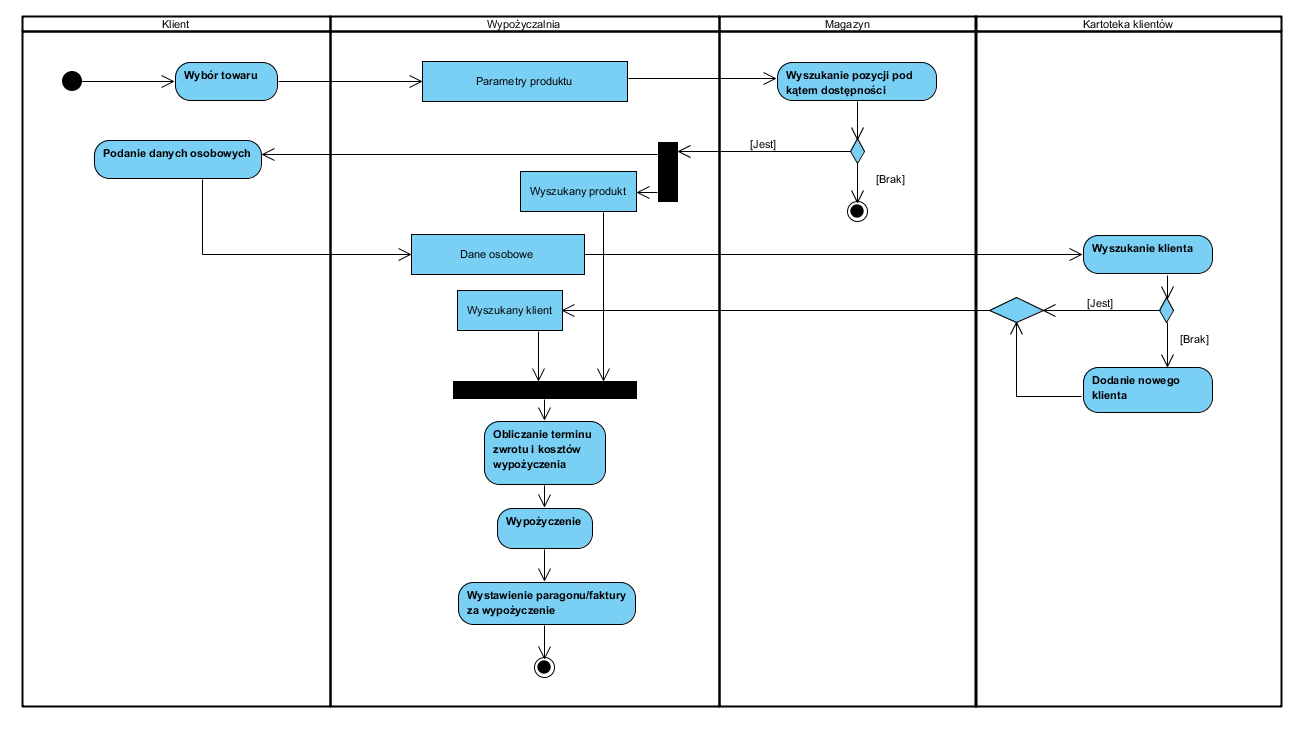
\includegraphics[height=10cm]{wypozyczenie.png}
	\caption{Stworzony diagram czynnści dla wypożyczenia}
	\label{fig:obrazek 1}
	\end{figure}

\newpage
	\subsubsection{Zwrot}
\begin{figure}[!ht]
	\centering
	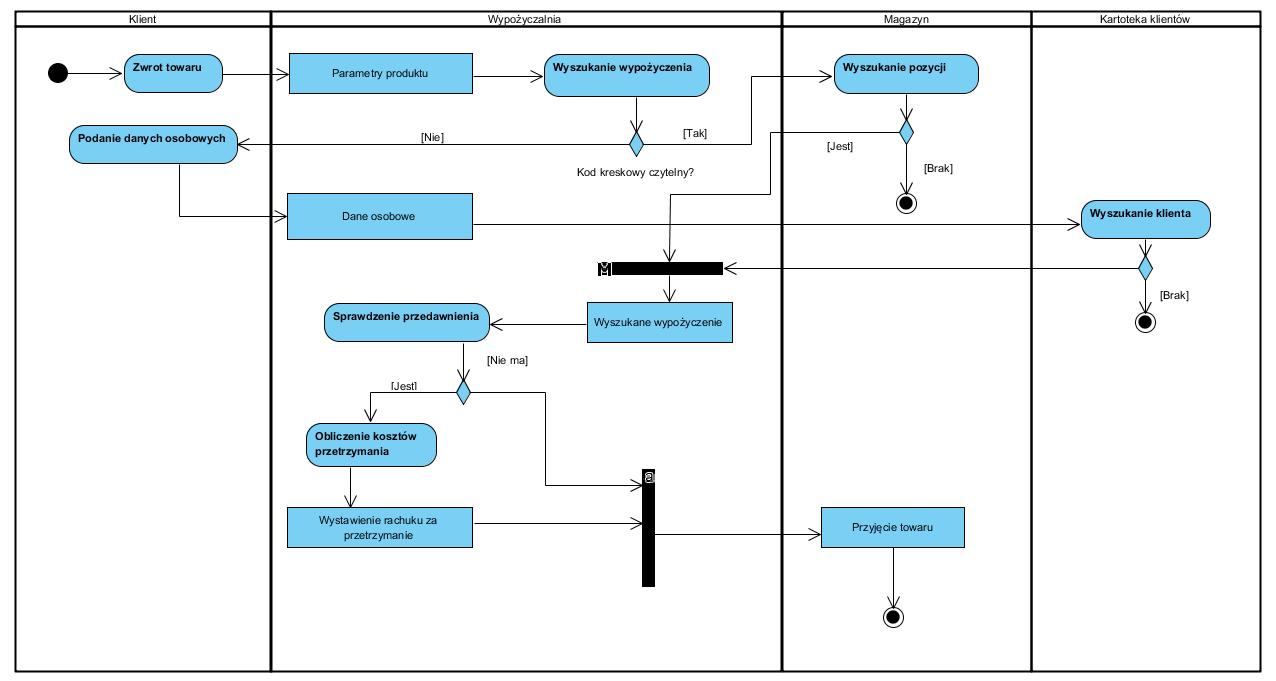
\includegraphics[height=9.5cm]{zwrot.png}
	\caption{Stworzony diagram czynności dla wypożyczenia}
	\label{fig:obrazek 2}
\end{figure}

	


\end{document}